\chapter{其他需求}

\section{数据库}
\subsection{文字说明}
本项目使用的数据库有如下几个表:
\begin{itemize}
	\item \textbf{用户表:}
	UID(主键),Uname,password,权限(普通用户,管理员),信用卡号,分享状态,当前IP
	\item \textbf{音乐表}:
	MID(主键),YID(外键),TID(外键),Mname,评价人数,平均分,总播放次数,风格ID,价格,路径(url)
	\item \textbf{艺人表:}
	YID(主键),Yname,性别,生日
	\item \textbf{评价表:}
	UID(主键),MID(主键),评分,评价内容(可以为空)
	\item \textbf{音乐表表:}
	TID,Tname,描述(char)
	\item \textbf{专辑表(音乐表表的子类):}
	TID(主键),YID(外键)
	\item \textbf{风格表(音乐表表的子表):}
	TID(主键)
	\item \textbf{购物车表(音乐表表的子表):}
	UID(主键,外键),
	\item \textbf{购买表(音乐表表的子表):}
	UID(主键,外键),TID
	\item \textbf{用户歌单表(音乐表表的子表):}
	UID(外键),TID(主键)
	\item \textbf{分享表:}
	RUID(主键,外键),CUID(外键),time,类别,ID(MID或TID)
	\item \textbf{连接表(音乐表和音乐之间):}
	TID,MID
\end{itemize}

本项目数据文件只有音乐文件。

数据库各个表说明如下:
\begin{itemize}
	\item \textbf{用户表:}存储用户的各种信息,其中未读分享状态标识用户是否有未读的分享信息。
	\item \textbf{歌曲表:}存储歌曲的各种信息,包括所属艺人,专辑,平均分等等。
	\item \textbf{艺人表:}艺人的各种信息。
	\item \textbf{音乐表表:}音乐表的表,专辑表,风格表,用户歌单,购物车,购买表都是音乐表的一种,上述表都是音乐表表的子类。
	\item \textbf{连接表:}音乐表表和歌曲表是多对多的关系,用连接表来说明各个音乐表包含的音乐。
	\item \textbf{分享表}:RUID和CUID是被分享者和分享者的ID,time是分享时间,类别是专辑,歌单还是单曲。

\end{itemize}

\subsection{实体图}
本数据库实体图如下:\\
(ISA表示子类继承关系)
\begin{figure}[ht]
	\centering
	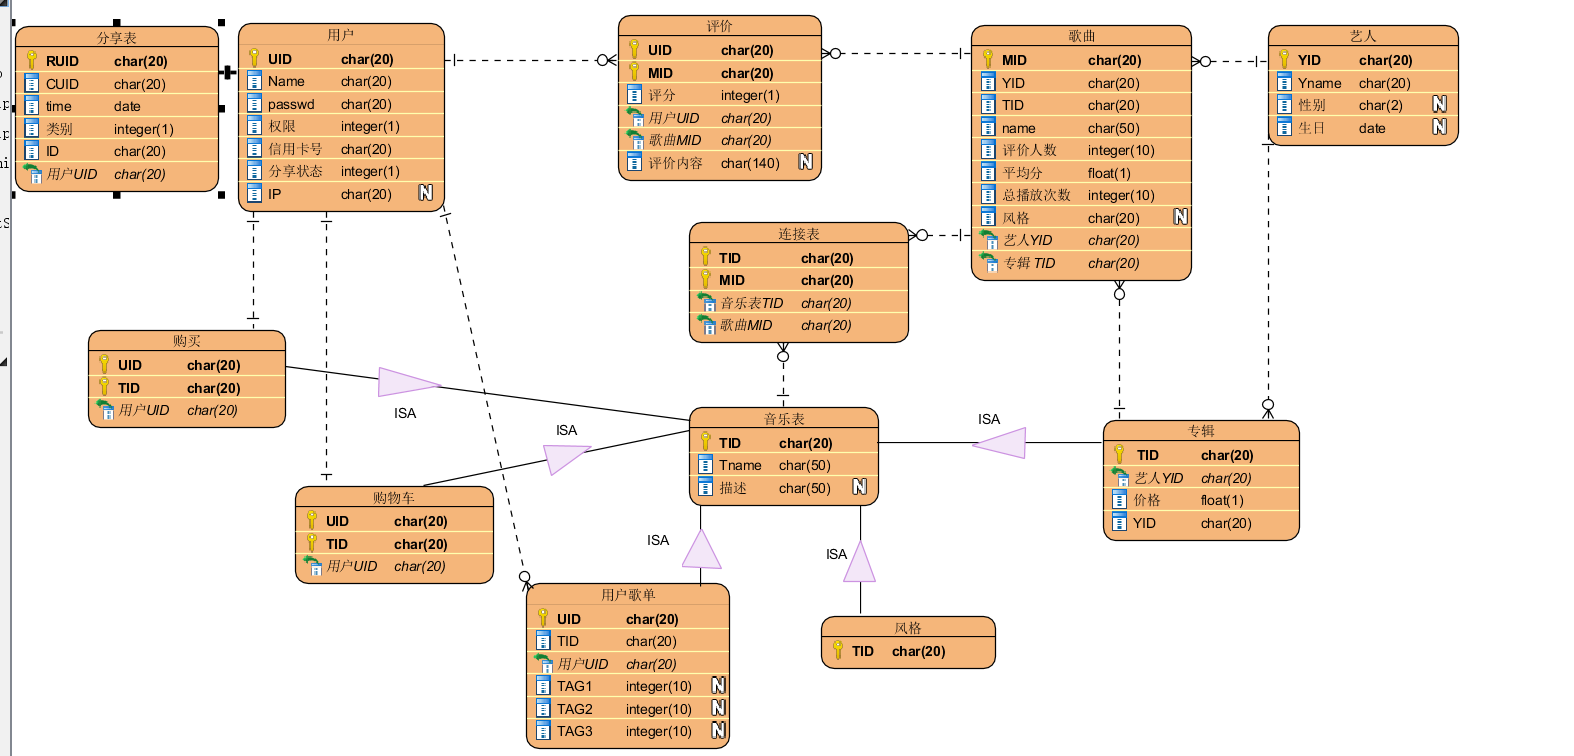
\includegraphics[width=10cm]{DataBase.png}
	\caption{数据库实体图} \label{fig:figure3}
	\end{figure}

\section{操作}

用户在不同的页面可以有不同的操作需求:
\begin{itemize}
	\item \textbf{登陆页面}
	\begin{itemize}
	\item \textbf{}1、输入账户名和密码。
	\item \textbf{}2、点击登录按钮跳转到用户主界面或者管理员页面。
	\item \textbf{}3、点击注册按钮跳转到注册页面。
	\end{itemize}
	\item \textbf{注册页面}
	\begin{itemize}
		\item \textbf{}1、输入新的自定义的账户名和密码。
		\item \textbf{}2、点击注册完成跳转到登录页面。
	\end{itemize}
	\item \textbf{用户主界面}
	\begin{itemize}
		\item \textbf{}1、点击注销按钮跳转到登录页面。
		\item \textbf{}2、点击浏览按钮跳转到浏览页面。
		\item \textbf{}3、点击推荐按钮跳转到推荐页面。
		\item \textbf{}4、点击任何一个歌单,查看歌单中的音乐。
		\item \textbf{}5、点击搜索跳转到搜索页面。
		\item \textbf{}6、点击排行榜跳转到排行榜页面。
		\item \textbf{}7、点击购物车跳转到购物车页面。
	\end{itemize}
	\item \textbf{歌单页面}
	\begin{itemize}
		\item \textbf{}1、删除歌单中的音乐。
		\item \textbf{}2、删除歌单
		\item \textbf{}3、分享歌单
	\end{itemize}
	\item \textbf{浏览页面}
	\begin{itemize}
		\item \textbf{}1、点击风格分类查看不同的风格的音乐。
		\item \textbf{}2、点击艺术家名字分类查看不同艺术家的音乐。
		\item \textbf{}3、点击不同专辑查看不同专辑中的音乐。
		\item \textbf{}4、点击音乐开始播放。
		\item \textbf{}5、点击加入购物车按钮将音乐加入购物车。
		\item \textbf{}6、点击添加到歌单按钮,选择歌单,将音乐添加到指定歌单。
		\item \textbf{}7、点击下载按钮,经过服务器判断有下载权限则下载到本地。
		\item \textbf{}8、点击分享按钮跳到分享页面。
	\end{itemize}
	\item \textbf{推荐页面}
	\begin{itemize}
		\item \textbf{}1、点击音乐开始播放播放页面。
		\item \textbf{}2、点击加入购物车按钮将音乐加入购物车。
		\item \textbf{}3、点击添加到歌单按钮,选择歌单,将音乐添加到指定歌单。
		\item \textbf{}4、点击下载按钮,经过服务器判断有下载权限则下载到本地。
		\item \textbf{}5、点击分享按钮跳到分享页面。
	\end{itemize}
	\item \textbf{搜索页面}
	\begin{itemize}
		\item \textbf{}1、在搜索框输入关键词。
		\item \textbf{}2、点击搜索按钮获取搜索结果。
		\item \textbf{}3、点击搜索出的音乐开始播放。
		\item \textbf{}4、点击加入购物车按钮将音乐加入购物车。
		\item \textbf{}5、点击添加到歌单按钮,选择歌单,将音乐添加到指定歌单。
		\item \textbf{}6、点击下载按钮,经过服务器判断有下载权限则下载到本地。
		\item \textbf{}7、点击分享按钮跳到分享页面。
	\end{itemize}
	\item \textbf{排行榜}
	\begin{itemize}
		\item \textbf{}1、点击音乐开始播放。
		\item \textbf{}2、点击加入购物车按钮将音乐加入购物车。
		\item \textbf{}3、点击添加到歌单按钮,选择歌单,将音乐添加到指定歌单。
		\item \textbf{}4、点击下载按钮,经过服务器判断有下载权限则下载到本地。
		\item \textbf{}5、点击分享按钮跳到分享页面。
	\end{itemize}
	\item \textbf{购物车:}
	\begin{itemize}
		\item \textbf{}1、点击删除按钮删除一个条目。
		\item \textbf{}2、点击结账按钮跳转到结算页面。
	\end{itemize}
	\item \textbf{结算页面:}
	\begin{itemize}
		\item \textbf{}1、点击结算按钮结账。
	\end{itemize}
	\item \textbf{播放页面:}
	\begin{itemize}
		\item \textbf{}1、点击播放按钮开始播放。
		\item \textbf{}2、点击暂停按钮暂停。
		\item \textbf{}3、点击下一首按钮进入跳转到下一首音乐的播放页面。
		\item \textbf{}4、点击上一首按钮进入跳转到上一首音乐的播放页面。
		\item \textbf{}5、点击评价评分。
		\item \textbf{}6、点击艺人查看对应艺人页面。
		\item \textbf{}7、点击专辑查看对应专辑页面。
	\end{itemize}
	\item \textbf{上传页面:}
	\begin{itemize}
		\item \textbf{}1、点击上传按钮,选择本地文件进行上传。上传完成后停留在上传页面。
	\end{itemize}
	\item \textbf{分享页面:}
	\begin{itemize}
		\item \textbf{}1、输入目标用户用户名,进行分享。
	\end{itemize}
\end{itemize}

\section{编码需求}
本项目要支持多种不同的编码,包括:ASCII,UTF-8,GB2312,Big5从而支持英文,简体中文和繁体中文的本地化工作。

\section{本地化}


本项目要为英文地区,简体中文地区和繁体中文地区做本地化工作。\\
本地化工程在初版软件开发完成后进行,本地化工程分为以下步骤:
\begin{itemize}
	\item\textbf{}(1)文件抽取与工作量统计;
	\item\textbf{}(2)文件格式转换与标记;
	\item\textbf{}(3)文件预翻译;
	\item\textbf{}(4) 检查并修正译文;
	\item\textbf{}(5) 生成本地化产品;
	\item\textbf{}(6) 修正产品的本地化缺陷;
	\item\textbf{}(7) 用户界面屏幕拍图;
	\item\textbf{}(8) 技术支持。
\end{itemize}


\section{错误处理}
	本项目应该对以下错误情况及时做出反应并正确提示用户:
	\begin{itemize}
		
	\item \textbf{}1、用户访问自己无权访问的信息时。
	\item \textbf{}	2、用户修改自己无权修改的信息时。
	\item \textbf{}3、用户使用的资源超出上限时。
	\item \textbf{}4、用户输入的信息错误时。
	\end{itemize}
	对于上述所有的错误情况,都要正确提示用户并且尽量不影响正序的正常运行。


\section{测试需求}
	本项目的测试需求包括:
\begin{itemize}
	
	\item \textbf{}1、测试所有已完成的功能可以正常运行。
	\item \textbf{}	2、测试所有错误处理能否正常运行,如用户输入错误账户密码等。
	\item \textbf{}	3、测试本项目在不同平台下的鲁棒性。
	\item \textbf{}4、测试本项目在用户大量访问时的可靠性。

\end{itemize}
	


